% Chapter 1: Introduction to Time Series Analysis
% Harvard-quality academic presentation
% Bachelor program, Bucharest University of Economic Studies

\documentclass[9pt, aspectratio=169, t]{beamer}

% Ensure content fits on slides
\setbeamersize{text margin left=8mm, text margin right=8mm}

%=============================================================================
% THEME AND STYLE CONFIGURATION
%=============================================================================
\usetheme{default}
% Using default theme for clean header/footer control

% Color Palette (matching Redispatch PDF)
\definecolor{MainBlue}{RGB}{26, 58, 110}
\definecolor{AccentBlue}{RGB}{26, 58, 110}
\definecolor{IDAred}{RGB}{205, 0, 0}
\definecolor{DarkGray}{RGB}{51, 51, 51}
\definecolor{MediumGray}{RGB}{128, 128, 128}
\definecolor{LightGray}{RGB}{248, 248, 248}
\definecolor{VeryLightGray}{RGB}{235, 235, 235}
\definecolor{KeynoteGray}{RGB}{218, 218, 218}
\definecolor{SectionGray}{RGB}{120, 120, 120}
\definecolor{FooterGray}{RGB}{100, 100, 100}
\definecolor{Crimson}{RGB}{220, 53, 69}
\definecolor{Forest}{RGB}{46, 125, 50}
\definecolor{Amber}{RGB}{181, 133, 63}
\definecolor{Orange}{RGB}{230, 126, 34}
\definecolor{Purple}{RGB}{142, 68, 173}

% Gradient background (exact Keynote 315° gradient: white to RGB 218,218,218)
\setbeamertemplate{background}{%
    \begin{tikzpicture}[remember picture, overlay]
        \shade[shading=axis, shading angle=315,
        top color=white, bottom color=KeynoteGray]
        (current page.south west) rectangle (current page.north east);
    \end{tikzpicture}%
}
% Fallback solid color for compatibility
\setbeamercolor{background canvas}{bg=}

\setbeamercolor{palette primary}{bg=MainBlue, fg=white}
\setbeamercolor{palette secondary}{bg=MainBlue!85, fg=white}
\setbeamercolor{palette tertiary}{bg=MainBlue!70, fg=white}
\setbeamercolor{structure}{fg=MainBlue}
\setbeamercolor{title}{fg=IDAred}
\setbeamercolor{frametitle}{fg=IDAred, bg=}
\setbeamercolor{block title}{bg=MainBlue, fg=white}
\setbeamercolor{block body}{bg=VeryLightGray, fg=DarkGray}
\setbeamercolor{block title alerted}{bg=Crimson, fg=white}
\setbeamercolor{block body alerted}{bg=Crimson!8, fg=DarkGray}
\setbeamercolor{block title example}{bg=Forest, fg=white}
\setbeamercolor{block body example}{bg=Forest!8, fg=DarkGray}
\setbeamercolor{item}{fg=MainBlue}

% Footer colors (override Madrid theme blue)
\setbeamercolor{author in head/foot}{fg=FooterGray, bg=}
\setbeamercolor{title in head/foot}{fg=FooterGray, bg=}
\setbeamercolor{date in head/foot}{fg=FooterGray, bg=}
\setbeamercolor{section in head/foot}{fg=FooterGray, bg=}
\setbeamercolor{subsection in head/foot}{fg=FooterGray, bg=}

% Bullet styles (apply everywhere including blocks)
\setbeamertemplate{itemize item}{\color{MainBlue}$\boxdot$}
\setbeamertemplate{itemize subitem}{\color{MainBlue}$\blacktriangleright$}
\setbeamertemplate{itemize subsubitem}{\color{MainBlue}\tiny$\bullet$}
\setbeamertemplate{itemize/enumerate body begin}{\normalsize}
\setbeamertemplate{itemize/enumerate subbody begin}{\normalsize}

% Item spacing
\setlength{\leftmargini}{1.5em}
\setlength{\leftmarginii}{1.5em}

\setbeamertemplate{navigation symbols}{}

%=============================================================================
% CUSTOM HEADLINE
%=============================================================================
\setbeamertemplate{headline}{%
    \vskip10pt%
    \hbox to \paperwidth{%
        \hskip0.5cm%
        {\small\color{FooterGray}\renewcommand{\hyperlink}[2]{##2}\insertsectionhead}%
        \hfill%
        \textcolor{FooterGray}{\small\insertframenumber}%
        \hskip0.5cm%
    }%
    \vskip4pt%
    {\color{FooterGray}\hrule height 0.4pt}%
}

%=============================================================================
% CUSTOM FOOTER
%=============================================================================
\usepackage{fontawesome5}

\setbeamertemplate{footline}{%
    {\color{FooterGray}\hrule height 0.4pt}%
    \vskip4pt%
    \hbox to \paperwidth{%
        \hskip0.5cm%
        \textcolor{FooterGray}{\small Time Series Analysis and Forecasting}%
        \hfill%
        \raisebox{-0.1em}{%
            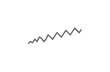
\begin{tikzpicture}[x=0.08em, y=0.08em, line width=0.4pt]
                \draw[FooterGray] (0,3) -- (1,4) -- (2,3.5) -- (3,5) -- (4,4) -- (5,6) -- (6,5.5) -- (7,4) -- (8,5) -- (9,7) -- (10,6) -- (11,5) -- (12,6.5) -- (13,8) -- (14,7) -- (15,6) -- (16,7.5) -- (17,9) -- (18,8) -- (19,7) -- (20,8.5) -- (21,10) -- (22,9) -- (23,8) -- (24,9.5);
            \end{tikzpicture}%
        }%
        \hskip0.5cm%
    }%
    \vskip6pt%
}

%=============================================================================
% PACKAGES
%=============================================================================
\usepackage[utf8]{inputenc}
\usepackage[T1]{fontenc}
\usepackage{amsmath, amssymb, amsthm}
\usepackage{mathtools}
\usepackage{bm}
\usepackage{tikz}
\usetikzlibrary{arrows.meta, positioning, shapes, calc, decorations.pathreplacing, shadings}
\usepackage{booktabs}
\usepackage{multirow}
\usepackage{array}
\usepackage{graphicx}
\usepackage{hyperref}
\usepackage{colortbl}
\hypersetup{colorlinks=true, linkcolor=MainBlue, urlcolor=MainBlue}
\graphicspath{{../logos/}{../charts/}}
\hfuzz=2pt  % Suppress tiny overfull warnings (<2pt)

%=============================================================================
% QUANTLET COMMAND
%=============================================================================
\newcommand{\quantlet}[2]{%
    \hfill\href{#2}{%
        \raisebox{-0.15em}{\includegraphics[height=0.7em]{ql_logo.png}}%
        \textcolor{MainBlue}{\tiny\ #1}%
    }%
}

%=============================================================================
% CUSTOM TITLE PAGE
%=============================================================================
\defbeamertemplate*{title page}{hybrid}[1][]
{
    \vspace{0.2cm}
    % Logos row - top header (with clickable links)
    \noindent\resizebox{\textwidth}{!}{%
        \href{https://www.ase.ro}{\includegraphics[height=1.0cm]{ase_logo.png}}\hspace{0.3cm}%
        \href{https://theida.net}{\includegraphics[height=1.0cm]{ida_logo.png}}\hspace{0.3cm}%
        \href{https://blockchain-research-center.com}{\includegraphics[height=1.0cm]{brc_logo.png}}\hspace{0.3cm}%
        \href{https://www.ai4efin.ase.ro}{\includegraphics[height=1.0cm]{ai4efin_logo.png}}\hspace{0.3cm}%
        \href{https://ipe.ro/new}{\includegraphics[height=1.0cm]{acad_logo.png}}\hspace{0.3cm}%
        \href{https://www.digital-finance-msca.com}{\includegraphics[height=1.0cm]{msca_logo.png}}%
    }

    \vspace{0.6cm}

    % Main title with Q logos on sides (with clickable links)
    \begin{center}
        \begin{minipage}{0.1\textwidth}
            \centering
            \href{https://quantlet.com}{\includegraphics[height=1.1cm]{ql_logo.png}}
        \end{minipage}%
        \begin{minipage}{0.78\textwidth}
            \centering
            {\LARGE\bfseries\usebeamercolor[fg]{title}\inserttitle}

            \vspace{0.3cm}

            {\usebeamerfont{subtitle}\usebeamercolor[fg]{title}\insertsubtitle}
        \end{minipage}%
        \begin{minipage}{0.1\textwidth}
            \centering
            \href{https://quantinar.com}{\includegraphics[height=1.1cm]{qr_logo.png}}
        \end{minipage}
    \end{center}

    \vspace{0.6cm}

    % Authors (left aligned)
    \hspace{0.5cm}{\usebeamerfont{author}\insertauthor}

    \vspace{0.3cm}

    % Institute/Affiliations (left aligned)
    \hspace{0.5cm}\begin{minipage}[t]{0.9\textwidth}
        \raggedright\small\insertinstitute
    \end{minipage}
}

%=============================================================================
% THEOREM ENVIRONMENTS
%=============================================================================
\theoremstyle{definition}
\setbeamertemplate{theorems}[numbered]
\newtheorem{defn}{Definition}
\newtheorem{thm}{Theorem}
\newtheorem{prop}{Proposition}
\newtheorem{rmk}{Remark}

%=============================================================================
% CUSTOM COMMANDS
%=============================================================================
\newcommand{\E}{\mathbb{E}}
\newcommand{\Var}{\text{Var}}
\newcommand{\Cov}{\text{Cov}}
\newcommand{\Corr}{\text{Corr}}
\newcommand{\R}{\mathbb{R}}
\newcommand{\N}{\mathbb{N}}
\newcommand{\Z}{\mathbb{Z}}
\newcommand{\RMSE}{\text{RMSE}}
\newcommand{\MAE}{\text{MAE}}
\newcommand{\MAPE}{\text{MAPE}}

%=============================================================================
% TITLE INFORMATION
%=============================================================================
\title[Time Series Analysis]{Time Series Analysis and Forecasting}
\subtitle{Chapter 0: Fundamentals}
\author[D.T. Pele]{Daniel Traian PELE}
\institute{Bucharest University of Economic Studies\\
IDA Institute Digital Assets\\
Blockchain Research Center\\
AI4EFin Artificial Intelligence for Energy Finance\\
Romanian Academy, Institute for Economic Forecasting\\
MSCA Digital Finance}
\date{}

\begin{document}

% Title page (no header/footer)
{
\setbeamertemplate{headline}{}
\setbeamertemplate{footline}{}
\begin{frame}
    \titlepage
\end{frame}
}

%=============================================================================
% COURSE OBJECTIVES
%=============================================================================
\begin{frame}{Learning Objectives}
    \textbf{\large By the end of this chapter, you will be able to:}
    \vspace{0.15cm}
    \begin{enumerate}
        \item[\textcolor{MainBlue}{\textbf{1.}}] \textbf{Define} time series and distinguish from cross-sectional and panel data
        \vspace{0.08cm}
        \item[\textcolor{MainBlue}{\textbf{2.}}] \textbf{Decompose} time series into trend-cycle, seasonal, and residual components
        \vspace{0.08cm}
        \item[\textcolor{MainBlue}{\textbf{3.}}] \textbf{Apply} exponential smoothing methods (SES, Holt, Holt-Winters, ETS)
        \vspace{0.08cm}
        \item[\textcolor{MainBlue}{\textbf{4.}}] \textbf{Evaluate} forecasts using MAE, RMSE, MAPE, sMAPE
        \vspace{0.08cm}
        \item[\textcolor{MainBlue}{\textbf{5.}}] \textbf{Implement} train/validation/test splits and cross-validation
        \vspace{0.08cm}
        \item[\textcolor{MainBlue}{\textbf{6.}}] \textbf{Model} seasonality using dummy variables or Fourier terms
        \vspace{0.08cm}
        \item[\textcolor{MainBlue}{\textbf{7.}}] \textbf{Remove} trend and seasonality through appropriate methods
        \vspace{0.08cm}
        \item[\textcolor{MainBlue}{\textbf{8.}}] \textbf{Distinguish} between deterministic and stochastic trends
    \end{enumerate}
\end{frame}

%=============================================================================
% TABLE OF CONTENTS
%=============================================================================
\begin{frame}{Chapter Outline}
    \setbeamertemplate{section in toc}{\color{MainBlue}$\boxdot$~\inserttocsection}
    \tableofcontents
\end{frame}

%=============================================================================
% MOTIVATION
%=============================================================================
\section{Motivation}

\begin{frame}{Time Series Are Everywhere}
    \vspace{-0.3cm}
    \begin{center}
        \includegraphics[width=0.95\textwidth, height=0.65\textheight, keepaspectratio]{ch1_motivation_everywhere.pdf}
    \end{center}
    \vspace{-0.2cm}
    {\footnotesize
    \begin{itemize}
        \item \textbf{Finance}: Stock prices, exchange rates, trading volumes
        \item \textbf{Economics}: GDP, unemployment, inflation rates
        \item \textbf{Business}: Sales, website traffic, customer demand
        \item \textbf{Science}: Temperature, pollution levels, patient vitals
    \end{itemize}
    }\quantlet{TSA\_ch1\_motivation}{https://github.com/QuantLet/TSA/tree/main/TSA_ch1/TSA_ch1_motivation}
\end{frame}

\begin{frame}{Why Study Time Series?}
    \vspace{-0.2cm}
    \begin{center}
        \includegraphics[width=0.95\textwidth, height=0.65\textheight, keepaspectratio]{ch1_motivation_forecast.pdf}
    \end{center}
    \vspace{-0.3cm}
    {\footnotesize
    \begin{alertblock}{Key Goal: Forecasting}
        Use historical patterns to predict future values --- critical for business planning, risk management, and policy decisions.
    \end{alertblock}
    }\quantlet{TSA\_ch1\_forecast}{https://github.com/QuantLet/TSA/tree/main/TSA_ch1/TSA_ch1_forecast}
\end{frame}

\begin{frame}{Understanding Time Series Structure}
    \vspace{-0.2cm}
    \begin{center}
        \includegraphics[width=0.95\textwidth, height=0.65\textheight, keepaspectratio]{ch1_motivation_components.pdf}
    \end{center}
    \vspace{-0.3cm}
    {\footnotesize
    \begin{exampleblock}{Decomposition}
        Every time series can be decomposed into interpretable components: trend-cycle, seasonality, and noise.
    \end{exampleblock}
    }\quantlet{TSA\_ch1\_components}{https://github.com/QuantLet/TSA/tree/main/TSA_ch1/TSA_ch1_components}
\end{frame}

%=============================================================================
% SECTION 1: WHAT IS A TIME SERIES
%=============================================================================
\section{What is a Time Series?}

\begin{frame}{Definition of a Time Series}
    \begin{defn}[Time Series]
        A \textbf{time series} is a sequence of observations $\{X_t\}$ indexed by time:
        \[
            \{X_t : t \in \mathcal{T}\}
        \]
        where $\mathcal{T}$ is an index set representing time points.
    \end{defn}

    \vspace{0.2cm}

    \begin{columns}[T]
        \column{0.5\textwidth}
        \begin{block}{Key Characteristics}
            \begin{itemize}
                \item \textbf{Ordered}: Natural temporal ordering
                \item \textbf{Dependent}: Consecutive observations correlated
                \item \textbf{Discrete/Continuous}: $t = 1, 2, 3, \ldots$
            \end{itemize}
        \end{block}

        \column{0.5\textwidth}
        \begin{exampleblock}{Notation}
            \begin{itemize}
                \item $X_t$ = observation at time $t$
                \item $\{X_t\}_{t=1}^{T}$ = series with $T$ observations
            \end{itemize}
        \end{exampleblock}
    \end{columns}
\end{frame}

\begin{frame}{Time Series: Visual Illustration}
    \begin{columns}[T]
        \column{0.35\textwidth}
        \begin{exampleblock}{Interpretation}
            Each point $X_t$ represents an observation at time $t$. The sequence is ordered and consecutive observations are typically correlated.
        \end{exampleblock}
        \vspace{0.3cm}
        \quantlet{TSA\_ch1\_def\_timeseries}{https://github.com/QuantLet/TSA/tree/main/TSA_ch1/TSA_ch1_def_timeseries}
        \column{0.63\textwidth}
        \vspace{-0.3cm}
        \begin{center}
            \includegraphics[width=\textwidth, height=0.78\textheight, keepaspectratio]{ch1_def_timeseries.pdf}
        \end{center}
    \end{columns}
\end{frame}

\begin{frame}{Common Time Series Patterns}
    \begin{columns}[T]
        \column{0.38\textwidth}
        \begin{block}{Pattern Types}
            \begin{itemize}
                \item \textbf{Trend}: Long-term increase or decrease
                \item \textbf{Seasonal}: Regular periodic patterns
                \item \textbf{Cyclical}: Medium-term fluctuations (2--10 years)
                \item \textbf{Random}: Unpredictable fluctuations
            \end{itemize}
        \end{block}
        \column{0.60\textwidth}
        \vspace{-0.3cm}
        \begin{center}
            \includegraphics[width=\textwidth, height=0.80\textheight, keepaspectratio]{ch1_ts_patterns.pdf}
        \end{center}
    \end{columns}
    \quantlet{TSA\_ch1\_patterns}{https://github.com/QuantLet/TSA/tree/main/TSA_ch1/TSA_ch1_patterns}
\end{frame}

\begin{frame}{Time Series: Visual Definition}
    \begin{columns}[T]
        \column{0.35\textwidth}
        \begin{block}{Interpretation}
            Each point $X_t$ represents a measurement at discrete time $t$. The temporal ordering creates dependence between observations. Data: S\&P 500 (2024).
        \end{block}
        \vspace{0.3cm}
        \quantlet{TSA\_ch1\_definition}{https://github.com/QuantLet/TSA/tree/main/TSA_ch1/TSA_ch1_definition}
        \column{0.63\textwidth}
        \vspace{-0.3cm}
        \begin{center}
            \includegraphics[width=\textwidth, height=0.78\textheight, keepaspectratio]{timeseries_definition.pdf}
        \end{center}
    \end{columns}
\end{frame}

\begin{frame}{Types of Data: Comparison}
    \begin{center}
        \includegraphics[width=0.95\textwidth, height=0.55\textheight, keepaspectratio]{data_types_comparison.pdf}
    \end{center}
    \vspace{-0.2cm}
    \begin{center}
    \small
    \begin{tabular}{lccc}
        \toprule
        \textbf{Data Type} & \textbf{Units ($N$)} & \textbf{Time ($T$)} & \textbf{Example} \\
        \midrule
        Cross-sectional & Many & 1 & Survey of 1000 households \\
        Time series & 1 & Many & Daily S\&P 500 prices \\
        Panel & Many & Many & GDP of 50 countries, 20 years \\
        \bottomrule
    \end{tabular}
    \end{center}
    \quantlet{TSA\_ch1\_data\_types}{https://github.com/QuantLet/TSA/tree/main/TSA_ch1/TSA_ch1_data_types}
\end{frame}

\begin{frame}{Examples of Time Series Data}
    \begin{columns}[T]
        \column{0.35\textwidth}
        \begin{exampleblock}{Real Financial Data}
            Yahoo Finance (2019--2025), normalized to base 100. Notice different volatility patterns: Bitcoin most volatile, Gold most stable.
        \end{exampleblock}
        \vspace{0.3cm}
        \quantlet{TSA\_ch1\_examples}{https://github.com/QuantLet/TSA/tree/main/TSA_ch1/TSA_ch1_examples}
        \column{0.63\textwidth}
        \vspace{-0.3cm}
        \begin{center}
            \includegraphics[width=\textwidth, height=0.78\textheight, keepaspectratio]{multiple_assets.pdf}
        \end{center}
    \end{columns}
\end{frame}

%=============================================================================
% SECTION 2: TIME SERIES DECOMPOSITION
%=============================================================================
\section{Time Series Decomposition}

\begin{frame}{Why Decompose a Time Series?}
    \textbf{Decomposition} separates a time series into interpretable components:

    \vspace{0.15cm}

    \begin{columns}[T]
        \begin{column}{0.48\textwidth}
            \textbf{Goals:}
            \begin{itemize}
                \item Understand underlying patterns
                \item Remove seasonality for modeling
                \item Identify trend direction
                \item Isolate irregular fluctuations
                \item Improve forecasting accuracy
            \end{itemize}
        \end{column}
        \begin{column}{0.48\textwidth}
            \textbf{Components:}
            \begin{itemize}
                \item $T_t$ = \textbf{Trend-Cycle}: Long-term movement
                \item $S_t$ = \textbf{Seasonal}: Regular periodic pattern
                \item $\varepsilon_t$ = \textbf{Residual}: Random noise
            \end{itemize}
            {\footnotesize\textit{Note: Cyclical component is typically absorbed into $T_t$}}
        \end{column}
    \end{columns}

    \vspace{0.2cm}

    \begin{block}{Classical Decomposition Models}
        \begin{itemize}
            \item \textbf{Additive}: $X_t = T_t + S_t + \varepsilon_t$
            \item \textbf{Multiplicative}: $X_t = T_t \times S_t \times \varepsilon_t$
        \end{itemize}
    \end{block}
\end{frame}

\begin{frame}{Time Series Decomposition: Visual Example}
    \vspace{-0.2cm}
    \begin{center}
        \includegraphics[width=0.95\textwidth, height=0.48\textheight, keepaspectratio]{ch1_decomposition.pdf}
    \end{center}
    \vspace{-0.3cm}
    {\small
    \begin{block}{Components Explained}
        \begin{itemize}
            \item \textbf{Original}: observed series
            \item \textbf{Trend-Cycle}: long-term movement
            \item \textbf{Seasonal}: periodic pattern
            \item \textbf{Residual}: random noise
        \end{itemize}
    \end{block}
    }\quantlet{TSA\_ch1\_decomposition}{https://github.com/QuantLet/TSA/tree/main/TSA_ch1/TSA_ch1_decomposition}
\end{frame}

\begin{frame}{The Cyclical Component}
    \vspace{-0.3cm}
    \begin{center}
        \includegraphics[width=0.95\textwidth, height=0.55\textheight, keepaspectratio]{ch1_cyclical_component.pdf}
    \end{center}
    \vspace{-0.2cm}
    {\small
    \begin{columns}[T]
        \column{0.48\textwidth}
        \begin{block}{Characteristics}
            \begin{itemize}
                \item Medium-term fluctuations (2--10 years)
                \item No fixed period (unlike seasonal)
                \item Reflects expansions/recessions
            \end{itemize}
        \end{block}

        \column{0.48\textwidth}
        \begin{alertblock}{In Practice}
            \begin{itemize}
                \item Cycle is often combined with trend
                \item Difficult to identify in short series
                \item Usually not modeled separately
            \end{itemize}
        \end{alertblock}
    \end{columns}
    }\quantlet{TSA\_ch1\_cyclical}{https://github.com/QuantLet/TSA/tree/main/TSA_ch1/TSA_ch1_cyclical}
\end{frame}

\begin{frame}{Additive Decomposition Model}
    \begin{block}{Model}
        \vspace{-0.3cm}
        \begin{equation}
            X_t = T_t + S_t + \varepsilon_t
        \end{equation}
        \vspace{-0.3cm}
    \end{block}

    \vspace{0.2cm}

    \begin{columns}[T]
        \column{0.48\textwidth}
        \begin{exampleblock}{When to Use}
            \begin{itemize}
                \item Seasonal fluctuations are \textbf{constant} over time
                \item Variance of the series is \textbf{stable}
            \end{itemize}
        \end{exampleblock}

        \column{0.48\textwidth}
        \begin{block}{Properties}
            \begin{itemize}
                \item $\E[\varepsilon_t] = 0$ (zero mean)
                \item $\sum_{j=1}^{s} S_j = 0$ (seasonal sums to zero)
                \item Units of $S_t$ same as $X_t$
            \end{itemize}
        \end{block}
    \end{columns}
\end{frame}

\begin{frame}{Additive Decomposition: US Retail Sales (FRED)}
    \vspace{-0.3cm}
    \begin{center}
        \includegraphics[width=0.95\textwidth, height=0.55\textheight, keepaspectratio]{ts_components_synthetic.pdf}
    \end{center}
    \vspace{-0.3cm}
    {\small
    \begin{block}{Interpretation}
        Original = Trend + Seasonal + Residual. Seasonal amplitude stays constant. Data: US Retail Sales (RSXFS) from FRED.
    \end{block}
    }\quantlet{TSA\_ch0\_additive}{https://github.com/QuantLet/TSA/tree/main/TSA_ch0/TSA_ch0_additive}
\end{frame}

\begin{frame}{Multiplicative Decomposition Model}
    \begin{block}{Model}
        \vspace{-0.3cm}
        \begin{equation}
            X_t = T_t \times S_t \times \varepsilon_t
        \end{equation}
        \vspace{-0.3cm}
    \end{block}

    \vspace{0.2cm}

    \begin{columns}[T]
        \column{0.48\textwidth}
        \begin{exampleblock}{When to Use}
            \begin{itemize}
                \item Seasonal fluctuations \textbf{grow} with series level
                \item Variance \textbf{increases} over time
            \end{itemize}
        \end{exampleblock}

        \column{0.48\textwidth}
        \begin{block}{Properties}
            \begin{itemize}
                \item $\E[\varepsilon_t] = 1$ (centered at 1)
                \item $\frac{1}{s}\sum S_j = 1$ (averages to 1)
                \item $S_t$ is dimensionless ratio
            \end{itemize}
        \end{block}
    \end{columns}

    \vspace{0.2cm}

    \begin{alertblock}{Tip}
        Log transform converts multiplicative to additive model: $\log X_t = \log T_t + \log S_t + \log \varepsilon_t$
    \end{alertblock}
\end{frame}

\begin{frame}{Multiplicative Decomposition: Real Data}
    \begin{columns}[T]
        \column{0.32\textwidth}
        \begin{exampleblock}{Example}
            Classic Box-Jenkins airline passengers (1949--1960). Seasonal amplitude grows with level.
        \end{exampleblock}
        \vspace{0.3cm}
        \quantlet{TSA\_ch0\_multiplicative}{https://github.com/QuantLet/TSA/tree/main/TSA_ch0/TSA_ch0_multiplicative}
        \column{0.66\textwidth}
        \vspace{-0.3cm}
        \begin{center}
            \includegraphics[width=\textwidth, height=0.80\textheight, keepaspectratio]{airline_decomposition.pdf}
        \end{center}
    \end{columns}
\end{frame}

\begin{frame}{Additive vs Multiplicative: Comparison}
    \begin{columns}[T]
        \column{0.35\textwidth}
        \begin{block}{Key Difference}
            \begin{itemize}
                \item \textbf{Multiplicative}: seasonal is a \textit{ratio} (centered at 1)
                \item \textbf{Additive}: seasonal in \textit{absolute units} (centered at 0)
            \end{itemize}
        \end{block}
        \vspace{0.3cm}
        \quantlet{TSA\_ch0\_comparison}{https://github.com/QuantLet/TSA/tree/main/TSA_ch0/TSA_ch0_comparison}
        \column{0.63\textwidth}
        \vspace{-0.3cm}
        \begin{center}
            \includegraphics[width=\textwidth, height=0.78\textheight, keepaspectratio]{additive_vs_multiplicative.pdf}
        \end{center}
    \end{columns}
\end{frame}

\begin{frame}{Trend Estimation: Moving Average}
    \begin{defn}[Centered Moving Average]
        The \textbf{centered moving average} of order $2q+1$ is:
        \vspace{-0.2cm}
        \begin{equation}
            \hat{T}_t = \frac{1}{2q+1} \sum_{j=-q}^{q} X_{t+j}
        \end{equation}
        \vspace{-0.3cm}
    \end{defn}

    \vspace{0.2cm}

    \begin{columns}[T]
        \column{0.48\textwidth}
        \begin{block}{For Seasonal Data}
            \begin{itemize}
                \item Period $s$ \textbf{odd}: simple average
                \item Period $s$ \textbf{even}: $2 \times s$ MA with half-weights
            \end{itemize}
        \end{block}

        \column{0.48\textwidth}
        \begin{exampleblock}{Properties}
            \begin{itemize}
                \item Smooths seasonal \& random
                \item Larger window $\Rightarrow$ smoother
                \item Trade-off: lose endpoints
            \end{itemize}
        \end{exampleblock}
    \end{columns}
\end{frame}

\begin{frame}{Centered Moving Average: Visual Illustration}
    \begin{columns}[T]
        \column{0.32\textwidth}
        \begin{exampleblock}{Interpretation}
            The moving average smooths out short-term fluctuations, revealing the underlying trend.
        \end{exampleblock}
        \vspace{0.3cm}
        \quantlet{TSA\_ch0\_ma}{https://github.com/QuantLet/TSA/tree/main/TSA_ch0/TSA_ch0_ma}
        \column{0.66\textwidth}
        \vspace{-0.3cm}
        \begin{center}
            \includegraphics[width=\textwidth, height=0.80\textheight, keepaspectratio]{ch1_def_moving_average.pdf}
        \end{center}
    \end{columns}
\end{frame}

\begin{frame}{Classical Decomposition Algorithm}
    \begin{block}{Steps for Multiplicative Decomposition}
        \begin{enumerate}
            \item \textbf{Estimate Trend}: $\hat{T}_t = MA_s(X_t)$
            \item \textbf{Detrend}: $D_t = X_t / \hat{T}_t$
            \item \textbf{Estimate Seasonal}: $\hat{S}_j = \text{mean}(D_t \text{ for season } j)$
            \item \textbf{Normalize}: Scale so $\frac{1}{s}\sum_{j=1}^{s} \hat{S}_j = 1$
            \item \textbf{Compute Residuals}: $\hat{\varepsilon}_t = X_t / (\hat{T}_t \times \hat{S}_t)$
        \end{enumerate}
    \end{block}

    \vspace{0.3cm}

    \begin{alertblock}{Note}
        For \textbf{additive} decomposition: replace division with subtraction and multiplication with addition.
    \end{alertblock}
\end{frame}

\begin{frame}{Seasonal Indices: Interpretation}
    \begin{columns}[T]
        \column{0.35\textwidth}
        \begin{exampleblock}{Interpretation}
            \begin{itemize}
                \item $S_t > 1$: above-average activity
                \item $S_t < 1$: below-average activity
                \item Airline data shows peak travel in July--August
            \end{itemize}
        \end{exampleblock}
        \vspace{0.3cm}
        \quantlet{TSA\_ch0\_seasonal}{https://github.com/QuantLet/TSA/tree/main/TSA_ch0/TSA_ch0_seasonal}
        \column{0.63\textwidth}
        \vspace{-0.3cm}
        \begin{center}
            \includegraphics[width=\textwidth, height=0.78\textheight, keepaspectratio]{seasonal_pattern.pdf}
        \end{center}
    \end{columns}
\end{frame}

\begin{frame}{STL Decomposition: A Modern Approach}
    \begin{defn}[STL - Seasonal-Trend decomposition using LOESS]
        \textbf{STL} uses locally weighted regression (LOESS): $X_t = T_t + S_t + R_t$
    \end{defn}

    \vspace{0.2cm}

    \begin{columns}[T]
        \column{0.5\textwidth}
        \begin{exampleblock}{Advantages}
            \begin{itemize}
                \item Any seasonal period
                \item Seasonal can change over time
                \item Robust to outliers
                \item Smooth trend estimates
            \end{itemize}
        \end{exampleblock}

        \column{0.5\textwidth}
        \begin{block}{Key Parameters}
            \begin{itemize}
                \item \texttt{period}: Seasonal period
                \item \texttt{seasonal}: Smoothing window
                \item \texttt{robust}: Downweight outliers
            \end{itemize}
        \end{block}
    \end{columns}
\end{frame}

\begin{frame}{STL Decomposition: Visual Illustration}
    \begin{columns}[T]
        \column{0.32\textwidth}
        \begin{block}{Key Insight}
            STL separates the series into trend, seasonal, and remainder using LOESS.
        \end{block}
        \vspace{0.3cm}
        \quantlet{TSA\_ch0\_stl}{https://github.com/QuantLet/TSA/tree/main/TSA_ch0/TSA_ch0_stl}
        \column{0.66\textwidth}
        \vspace{-0.3cm}
        \begin{center}
            \includegraphics[width=\textwidth, height=0.80\textheight, keepaspectratio]{ch1_def_stl.pdf}
        \end{center}
    \end{columns}
\end{frame}

%=============================================================================
% SECTION 3: EXPONENTIAL SMOOTHING METHODS
%=============================================================================
\section{Exponential Smoothing Methods}

\begin{frame}{Exponential Smoothing: Overview}
    \begin{block}{Definition}
        \textbf{Exponential smoothing} produces forecasts based on weighted averages of past observations, with weights decaying exponentially.
    \end{block}

    \vspace{0.2cm}

    \begin{columns}[T]
        \column{0.5\textwidth}
        \begin{exampleblock}{Why Exponential Smoothing?}
            \begin{itemize}
                \item Simple yet effective
                \item Recent obs. get higher weights
                \item Handles trend \& seasonality
                \item Foundation for ETS models
            \end{itemize}
        \end{exampleblock}

        \column{0.5\textwidth}
        \begin{alertblock}{Three Main Methods}
            \begin{enumerate}
                \item \textbf{SES}: Level only
                \item \textbf{Holt}: Level + Trend
                \item \textbf{Holt-Winters}: + Seasonality
            \end{enumerate}
        \end{alertblock}
    \end{columns}
\end{frame}

\begin{frame}{Moving Average Smoothing}
    \vspace{-0.2cm}
    \begin{center}
        \includegraphics[width=0.95\textwidth, height=0.60\textheight, keepaspectratio]{ch1_moving_average.pdf}
    \end{center}
    \vspace{-0.3cm}
    \begin{block}{Window Size Trade-off}
        \begin{itemize}
            \item \textbf{Small window}: Responsive but noisy
            \item \textbf{Large window}: Smoother but slower to react
        \end{itemize}
    \end{block}
    \quantlet{TSA\_ch1\_moving\_average}{https://github.com/QuantLet/TSA/tree/main/TSA_ch1/TSA_ch1_moving_average}
\end{frame}

\begin{frame}{Simple Exponential Smoothing (SES)}
    \begin{block}{Model}
        \vspace{-0.2cm}
        \begin{equation}
            \hat{X}_{t+1|t} = \alpha X_t + (1-\alpha)\hat{X}_{t|t-1}
        \end{equation}
        \vspace{-0.2cm}
        where $\alpha \in (0,1)$ is the \textbf{smoothing parameter}.
    \end{block}

    \vspace{0.2cm}

    \begin{columns}[T]
        \column{0.5\textwidth}
        \begin{exampleblock}{How It Works}
            \begin{itemize}
                \item Weights decay exponentially
                \item Large $\alpha$: responsive
                \item Small $\alpha$: smoother
            \end{itemize}
        \end{exampleblock}

        \column{0.5\textwidth}
        \begin{block}{Level Form}
            $$\ell_t = \alpha X_t + (1-\alpha)\ell_{t-1}$$
        \end{block}
    \end{columns}
\end{frame}

\begin{frame}{Simple Exponential Smoothing: Effect of $\alpha$}
    \begin{columns}[T]
        \column{0.32\textwidth}
        \begin{exampleblock}{Trade-off}
            Smaller $\alpha$ produces smoother forecasts; larger $\alpha$ follows data more closely.
        \end{exampleblock}
        \vspace{0.3cm}
        \quantlet{TSA\_ch0\_ses}{https://github.com/QuantLet/TSA/tree/main/TSA_ch0/TSA_ch0_ses}
        \column{0.66\textwidth}
        \vspace{-0.3cm}
        \begin{center}
            \includegraphics[width=\textwidth, height=0.80\textheight, keepaspectratio]{simple_exp_smoothing.pdf}
        \end{center}
    \end{columns}
\end{frame}

\begin{frame}{Holt's Linear Trend Method}
    \begin{block}{Equations}
        \begin{itemize}
            \item \textbf{Level:} $\ell_t = \alpha X_t + (1-\alpha)(\ell_{t-1} + b_{t-1})$
            \item \textbf{Trend:} $b_t = \beta^*(\ell_t - \ell_{t-1}) + (1-\beta^*)b_{t-1}$
            \item \textbf{Forecast:} $\hat{X}_{t+h|t} = \ell_t + h \cdot b_t$
        \end{itemize}
    \end{block}

    \vspace{0.2cm}

    \begin{columns}[T]
        \column{0.5\textwidth}
        \begin{exampleblock}{Parameters}
            \begin{itemize}
                \item $\alpha$: Level smoothing
                \item $\beta^*$: Trend smoothing
            \end{itemize}
        \end{exampleblock}

        \column{0.5\textwidth}
        \begin{block}{Components}
            \begin{itemize}
                \item $\ell_t$: Estimated level
                \item $b_t$: Estimated trend (slope)
            \end{itemize}
        \end{block}
    \end{columns}
\end{frame}

\begin{frame}{Holt's Method: Visualization}
    \begin{columns}[T]
        \column{0.35\textwidth}
        \begin{exampleblock}{Interpretation}
            \begin{itemize}
                \item Holt's method captures both level and trend
                \item Projects them into the forecast horizon
                \item $\alpha$ controls level changes
                \item $\beta^*$ controls trend changes
            \end{itemize}
        \end{exampleblock}
        \vspace{0.2cm}
        \quantlet{TSA\_ch0\_holt}{https://github.com/QuantLet/TSA/tree/main/TSA_ch0/TSA_ch0_holt}
        \column{0.63\textwidth}
        \vspace{-0.3cm}
        \begin{center}
            \includegraphics[width=\textwidth, height=0.78\textheight, keepaspectratio]{holt_method.pdf}
        \end{center}
    \end{columns}
\end{frame}

\begin{frame}{Holt-Winters Seasonal Method}
    \begin{block}{Equations (Additive Seasonality)}
        \begin{itemize}
            \item \textbf{Level:} $\ell_t = \alpha(X_t - S_{t-s}) + (1-\alpha)(\ell_{t-1} + b_{t-1})$
            \item \textbf{Trend:} $b_t = \beta^*(\ell_t - \ell_{t-1}) + (1-\beta^*)b_{t-1}$
            \item \textbf{Seasonal:} $S_t = \gamma(X_t - \ell_t) + (1-\gamma)S_{t-s}$
            \item \textbf{Forecast:} $\hat{X}_{t+h|t} = \ell_t + h \cdot b_t + S_{t+h-s(k+1)}$
        \end{itemize}
    \end{block}

    \vspace{0.2cm}

    \begin{exampleblock}{Parameters}
        \begin{itemize}
            \item $\alpha$: Level smoothing
            \item $\beta^*$: Trend smoothing
            \item $\gamma$: Seasonal smoothing
            \item $s$: Seasonal period
        \end{itemize}
    \end{exampleblock}
\end{frame}

\begin{frame}{Holt-Winters: Capturing Seasonality}
    \begin{columns}[T]
        \column{0.32\textwidth}
        \begin{exampleblock}{Key Feature}
            Holt-Winters decomposes the series and produces seasonal forecasts with trend.
        \end{exampleblock}
        \vspace{0.3cm}
        \quantlet{TSA\_ch0\_hw}{https://github.com/QuantLet/TSA/tree/main/TSA_ch0/TSA_ch0_hw}
        \column{0.66\textwidth}
        \vspace{-0.3cm}
        \begin{center}
            \includegraphics[width=\textwidth, height=0.80\textheight, keepaspectratio]{holt_winters.pdf}
        \end{center}
    \end{columns}
\end{frame}

\begin{frame}{ETS Framework: Error-Trend-Seasonal}
    \begin{defn}[ETS Models]
        The \textbf{ETS framework} generalizes exponential smoothing: ETS$(E, T, S)$
    \end{defn}

    \vspace{0.1cm}

    \begin{center}
    \begin{tabular}{llll}
        \toprule
        \textbf{Component} & \textbf{N} & \textbf{A} & \textbf{M} \\
        \midrule
        Error (E) & -- & Additive & Multiplicative \\
        Trend (T) & None & Additive & Multiplicative \\
        Seasonal (S) & None & Additive & Multiplicative \\
        \bottomrule
    \end{tabular}
    \end{center}

    \vspace{0.2cm}

    \begin{exampleblock}{Examples}
        \begin{itemize}
            \item ETS(A,N,N) = Simple Exponential Smoothing
            \item ETS(A,A,N) = Holt's Linear Method
            \item ETS(A,A,A) = Holt-Winters Additive
        \end{itemize}
    \end{exampleblock}
\end{frame}

\begin{frame}{ETS: Exponential Smoothing Illustration}
    \begin{columns}[T]
        \column{0.32\textwidth}
        \begin{exampleblock}{Interpretation}
            ETS models use exponentially weighted observations for forecasting. Weights decay as observations get older.
        \end{exampleblock}
        \vspace{0.3cm}
        \quantlet{TSA\_ch0\_ets}{https://github.com/QuantLet/TSA/tree/main/TSA_ch0/TSA_ch0_ets}
        \column{0.66\textwidth}
        \vspace{-0.3cm}
        \begin{center}
            \includegraphics[width=\textwidth, height=0.80\textheight, keepaspectratio]{ch1_def_ets.pdf}
        \end{center}
    \end{columns}
\end{frame}

\begin{frame}{ETS Model Selection}
    \begin{columns}[T]
        \column{0.32\textwidth}
        \begin{exampleblock}{Interpretation}
            The ETS framework provides a systematic way to choose the best model using AIC/BIC.
        \end{exampleblock}
        \vspace{0.3cm}
        \quantlet{TSA\_ch0\_ets\_select}{https://github.com/QuantLet/TSA/tree/main/TSA_ch0/TSA_ch0_ets_select}
        \column{0.66\textwidth}
        \vspace{-0.3cm}
        \begin{center}
            \includegraphics[width=\textwidth, height=0.80\textheight, keepaspectratio]{ets_components.pdf}
        \end{center}
    \end{columns}
\end{frame}

\begin{frame}{Damped Trend Methods}
    \begin{block}{Damping Parameter}
        Introduces $\phi \in (0,1)$ to prevent over-projection
    \end{block}

    \vspace{0.1cm}

    \begin{columns}[T]
        \column{0.55\textwidth}
        \begin{block}{Equations}
            \begin{itemize}
                \item \textbf{Level:} $\ell_t = \alpha X_t + (1-\alpha)(\ell_{t-1} + \phi b_{t-1})$
                \item \textbf{Trend:} $b_t = \beta^*(\ell_t - \ell_{t-1}) + (1-\beta^*)\phi b_{t-1}$
                \item \textbf{Forecast:} $\hat{X}_{t+h|t} = \ell_t + \phi\frac{1-\phi^h}{1-\phi}b_t$
            \end{itemize}
        \end{block}
        \column{0.43\textwidth}
        \begin{exampleblock}{Key Insight}
            \begin{itemize}
                \item As $h \to \infty$: forecast $\to$ constant
                \item Prevents unrealistic long-term extrapolation
                \item Often best for longer horizons
            \end{itemize}
        \end{exampleblock}
    \end{columns}
\end{frame}

%=============================================================================
% SECTION 4: FORECAST EVALUATION
%=============================================================================
\section{Forecast Evaluation}

\begin{frame}{Forecast Accuracy Metrics}
    \begin{block}{Forecast Error}
        \begin{itemize}
            \item $e_t = X_t - \hat{X}_t$ (actual minus predicted)
        \end{itemize}
    \end{block}

    \vspace{0.1cm}

    \begin{columns}[T]
        \begin{column}{0.48\textwidth}
            \begin{block}{Scale-Dependent}
                \begin{itemize}
                    \item MAE $= \frac{1}{n}\sum|e_t|$
                    \item MSE $= \frac{1}{n}\sum e_t^2$
                    \item RMSE $= \sqrt{\text{MSE}}$
                \end{itemize}
            \end{block}
        \end{column}
        \begin{column}{0.48\textwidth}
            \begin{block}{Scale-Independent}
                \begin{itemize}
                    \item MAPE $= \frac{100}{n}\sum\left|\frac{e_t}{X_t}\right|$
                    \item sMAPE $= \frac{100}{n}\sum\frac{|e_t|}{(|X_t|+|\hat{X}_t|)/2}$
                \end{itemize}
            \end{block}
        \end{column}
    \end{columns}

    \vspace{0.15cm}

    \begin{alertblock}{Which to use?}
        \begin{itemize}
            \item Same series: RMSE, MAE
            \item Compare across series: MAPE, sMAPE
        \end{itemize}
    \end{alertblock}
\end{frame}

\begin{frame}{Forecast Evaluation: Visual Example}
    \vspace{-0.2cm}
    \begin{center}
        \includegraphics[width=0.95\textwidth, height=0.62\textheight, keepaspectratio]{ch1_forecast_eval.pdf}
    \end{center}
    \vspace{-0.2cm}
    {\footnotesize
    \begin{itemize}
        \item \textbf{Top}: Actual values vs. forecasted values -- visual assessment of fit
        \item \textbf{Bottom}: Residuals should be centered around zero with no pattern
        \item Good forecasts have small, random residuals with constant variance
    \end{itemize}
    }\quantlet{TSA\_ch1\_forecast\_eval}{https://github.com/QuantLet/TSA/tree/main/TSA_ch1/TSA_ch1_forecast_eval}
\end{frame}

\begin{frame}{Comparing Forecast Methods}
    \vspace{-0.2cm}
    \begin{center}
        \includegraphics[width=0.95\textwidth, height=0.58\textheight, keepaspectratio]{forecast_accuracy_metrics.pdf}
    \end{center}
    \vspace{-0.3cm}
    \begin{exampleblock}{Interpretation}
        {\small
        \begin{itemize}
            \item \textbf{Left:} Comparing SES, Holt, and Holt-Winters forecasts
            \item \textbf{Right:} Error metrics for each method
        \end{itemize}
        }
    \end{exampleblock}
    \quantlet{TSA\_ch0\_forecast\_compare}{https://github.com/QuantLet/TSA/tree/main/TSA_ch0/TSA_ch0_forecast_compare}
\end{frame}

\begin{frame}{Residual Diagnostics}
    \begin{columns}[T]
        \column{0.48\textwidth}
        \begin{block}{Residual Properties}
            Good forecasts should have residuals that are:
            \begin{enumerate}
                \item \textbf{Zero mean}: $\E[e_t] = 0$
                \item \textbf{Uncorrelated}: $\Cov(e_t, e_{t-k}) = 0$
                \item \textbf{Constant variance}: $\Var(e_t) = \sigma^2$
                \item \textbf{Normally distributed}
            \end{enumerate}
        \end{block}
        \column{0.5\textwidth}
        \begin{exampleblock}{Diagnostic Tests}
            \textbf{Ljung-Box test} (autocorrelation):
            \[
                Q = T(T+2)\sum_{k=1}^{h}\frac{\hat{\rho}_k^2}{T-k} \sim \chi^2_h
            \]

            \textbf{Jarque-Bera test} (normality):
            \[
                JB = \frac{T}{6}\left(S^2 + \frac{(K-3)^2}{4}\right) \sim \chi^2_2
            \]
            {\small $S$ = skewness, $K$ = kurtosis}
        \end{exampleblock}
    \end{columns}
\end{frame}

\begin{frame}{Residual Diagnostics: Visualization}
    \begin{columns}[T]
        \column{0.32\textwidth}
        \begin{exampleblock}{What to Check}
            \begin{itemize}
                \item Time plot (no patterns)
                \item Histogram (normality)
                \item ACF (no autocorrelation)
                \item Q-Q plot (normality)
            \end{itemize}
        \end{exampleblock}
        \vspace{0.3cm}
        \quantlet{TSA\_ch0\_residuals}{https://github.com/QuantLet/TSA/tree/main/TSA_ch0/TSA_ch0_residuals}
        \column{0.66\textwidth}
        \vspace{-0.3cm}
        \begin{center}
            \includegraphics[width=\textwidth, height=0.80\textheight, keepaspectratio]{residual_diagnostics.pdf}
        \end{center}
    \end{columns}
\end{frame}

\begin{frame}{Time Series Cross-Validation}
    \begin{columns}[T]
        \begin{column}{0.48\textwidth}
            \begin{alertblock}{Why Not Standard CV?}
                \begin{itemize}
                    \item Time series have temporal dependence
                    \item Future data cannot predict the past
                    \item Standard k-fold causes data leakage
                \end{itemize}
            \end{alertblock}
        \end{column}
        \begin{column}{0.48\textwidth}
            \begin{block}{Rolling Origin CV}
                \begin{enumerate}
                    \item Train on $\{X_1, \ldots, X_t\}$
                    \item Forecast $\hat{X}_{t+h}$
                    \item Increment $t$, repeat
                \end{enumerate}
            \end{block}
        \end{column}
    \end{columns}

    \begin{center}
        \includegraphics[width=0.95\textwidth, height=0.42\textheight, keepaspectratio]{cross_validation_forecast.pdf}
    \end{center}
    \quantlet{TSA\_ch0\_cv}{https://github.com/QuantLet/TSA/tree/main/TSA_ch0/TSA_ch0_cv}
\end{frame}

\begin{frame}{Train / Validation / Test Split}
    \textbf{Three-way split} for model development:

    \vspace{0.2cm}

    \begin{columns}[T]
        \begin{column}{0.32\textwidth}
            \textbf{\textcolor{MainBlue}{Training Set}}
            \begin{itemize}
                \item Fit model parameters
                \item Largest portion (60--80\%)
                \item Used for estimation
            \end{itemize}
        \end{column}
        \begin{column}{0.32\textwidth}
            \textbf{\textcolor{Forest}{Validation Set}}
            \begin{itemize}
                \item Tune hyperparameters
                \item Compare models
                \item Select best approach
            \end{itemize}
        \end{column}
        \begin{column}{0.32\textwidth}
            \textbf{\textcolor{Crimson}{Test Set}}
            \begin{itemize}
                \item Final evaluation only
                \item Never used for tuning
                \item Unbiased performance
            \end{itemize}
        \end{column}
    \end{columns}

    \vspace{0.1cm}

    \begin{center}
        \includegraphics[width=0.75\textwidth, height=0.42\textheight, keepaspectratio]{train_test_validation.pdf}
    \end{center}
    \quantlet{TSA\_ch0\_train\_split}{https://github.com/QuantLet/TSA/tree/main/TSA_ch0/TSA_ch0_train_split}
\end{frame}

\begin{frame}{Model Development Workflow}
    \begin{center}
    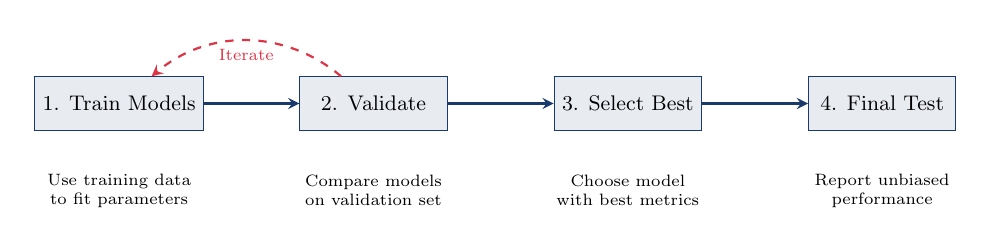
\begin{tikzpicture}[node distance=1.8cm, scale=0.85, transform shape]
        \tikzstyle{process} = [rectangle, minimum width=2.2cm, minimum height=0.8cm, text centered, draw=MainBlue, fill=MainBlue!10, font=\small]
        \tikzstyle{arrow} = [->, >=stealth, thick, MainBlue]

        % Nodes
        \node (train) [process] {1. Train Models};
        \node (validate) [process, right of=train, xshift=2cm] {2. Validate};
        \node (select) [process, right of=validate, xshift=2cm] {3. Select Best};
        \node (test) [process, right of=select, xshift=2cm] {4. Final Test};

        % Arrows
        \draw [arrow] (train) -- (validate);
        \draw [arrow] (validate) -- (select);
        \draw [arrow] (select) -- (test);

        % Feedback loop
        \draw [arrow, dashed, Crimson] (validate) to[bend right=40] node[below, font=\scriptsize] {Iterate} (train);

        % Labels below
        \node [below of=train, yshift=0.5cm, font=\scriptsize, text width=2.5cm, align=center] {Use training data\\to fit parameters};
        \node [below of=validate, yshift=0.5cm, font=\scriptsize, text width=2.5cm, align=center] {Compare models\\on validation set};
        \node [below of=select, yshift=0.5cm, font=\scriptsize, text width=2.5cm, align=center] {Choose model\\with best metrics};
        \node [below of=test, yshift=0.5cm, font=\scriptsize, text width=2.5cm, align=center] {Report unbiased\\performance};
    \end{tikzpicture}
    \end{center}

    \vspace{0.15cm}

    \begin{alertblock}{Critical Rule}
        \textbf{Never} use test set for model selection! This causes \textit{data leakage} and overly optimistic performance estimates.
    \end{alertblock}
\end{frame}

\begin{frame}{Real Data: Forecast Comparison}
    \begin{columns}[T]
        \column{0.32\textwidth}
        \begin{exampleblock}{Interpretation}
            Airline passengers data: Holt-Winters Multiplicative performs best for seasonal data.
        \end{exampleblock}
        \vspace{0.3cm}
        \quantlet{TSA\_ch0\_real\_data}{https://github.com/QuantLet/TSA/tree/main/TSA_ch0/TSA_ch0_real_data}
        \column{0.66\textwidth}
        \vspace{-0.3cm}
        \begin{center}
            \includegraphics[width=\textwidth, height=0.80\textheight, keepaspectratio]{real_data_forecast_comparison.pdf}
        \end{center}
    \end{columns}
\end{frame}

\begin{frame}{Forecast Performance Across Datasets}
    \begin{columns}[T]
        \column{0.32\textwidth}
        \begin{exampleblock}{Interpretation}
            Different series require different models. Seasonal data needs seasonal methods.
        \end{exampleblock}
        \vspace{0.3cm}
        \quantlet{TSA\_ch0\_multi\_series}{https://github.com/QuantLet/TSA/tree/main/TSA_ch0/TSA_ch0_multi_series}
        \column{0.66\textwidth}
        \vspace{-0.3cm}
        \begin{center}
            \includegraphics[width=\textwidth, height=0.80\textheight, keepaspectratio]{multiple_series_comparison.pdf}
        \end{center}
    \end{columns}
\end{frame}

%=============================================================================
% SECTION 5: MODELING SEASONALITY
%=============================================================================
\section{Modeling Seasonality}

\begin{frame}{Modeling Seasonality: Two Approaches}
    \begin{columns}[T]
        \begin{column}{0.48\textwidth}
            \textbf{1. Dummy Variables:}

            \vspace{0.1cm}
            $X_t = \mu + \sum_{j=1}^{s-1}\gamma_j D_{jt} + \varepsilon_t$

            \vspace{0.2cm}
            \begin{itemize}
                \item $D_{jt} = 1$ if $t$ in season $j$
                \item $s-1$ parameters
                \item Any seasonal pattern
            \end{itemize}
        \end{column}
        \begin{column}{0.48\textwidth}
            \textbf{2. Fourier Terms:}

            \vspace{0.1cm}
            $X_t = \mu + \sum_{k=1}^{K}[\alpha_k\sin(\cdot) + \beta_k\cos(\cdot)]$

            \vspace{0.2cm}
            \begin{itemize}
                \item Sinusoidal functions
                \item $2K$ parameters
                \item Smooth patterns
            \end{itemize}
        \end{column}
    \end{columns}

    \vspace{0.15cm}

    \begin{alertblock}{Trade-off}
        \begin{itemize}
            \item \textbf{Dummies}: any pattern, more parameters
            \item \textbf{Fourier}: smooth, fewer parameters
        \end{itemize}
    \end{alertblock}
\end{frame}

\begin{frame}{Dummy Variables vs Fourier Terms}
    \begin{columns}[T]
        \column{0.35\textwidth}
        \begin{block}{Comparison}
            \begin{itemize}
                \item \textbf{Dummies}: capture any shape but need $s-1$ parameters
                \item \textbf{Fourier}: uses $2K$ parameters for smooth patterns
            \end{itemize}
        \end{block}
        \vspace{0.3cm}
        \quantlet{TSA\_ch0\_fourier}{https://github.com/QuantLet/TSA/tree/main/TSA_ch0/TSA_ch0_fourier}
        \column{0.63\textwidth}
        \vspace{-0.3cm}
        \begin{center}
            \includegraphics[width=\textwidth, height=0.78\textheight, keepaspectratio]{seasonality_fourier_dummies.pdf}
        \end{center}
    \end{columns}
\end{frame}

\begin{frame}{Choosing Between Dummies and Fourier}
    \begin{center}
    \small
    \begin{tabular}{lcc}
        \toprule
        \textbf{Criterion} & \textbf{Dummies} & \textbf{Fourier} \\
        \midrule
        Parameters (monthly) & 11 & $2K$ (often 4--6) \\
        Seasonal pattern & Any shape & Smooth/sinusoidal \\
        Interpretation & Direct (month effects) & Frequency components \\
        High-frequency seasons & Many parameters & Efficient \\
        Multiple seasonality & Complex & Easy (add terms) \\
        \bottomrule
    \end{tabular}
    \end{center}

    \vspace{0.1cm}

    \begin{exampleblock}{Guidelines}
        \begin{itemize}
            \item Use \textbf{dummies}: irregular patterns, interpretable coefficients
            \item Use \textbf{Fourier}: smooth patterns, high-frequency seasonality, multiple periods
            \item \textbf{Fourier terms} are used in TBATS and Facebook Prophet
        \end{itemize}
    \end{exampleblock}
\end{frame}

%=============================================================================
% SECTION 6: HANDLING TREND AND SEASONALITY
%=============================================================================
\section{Handling Trend and Seasonality}

\begin{frame}{Why Remove Trend and Seasonality?}
    \textbf{Before modeling}, we often need to make series stationary:

    \vspace{0.15cm}

    \begin{columns}[T]
        \begin{column}{0.48\textwidth}
            \textbf{Reasons to detrend:}
            \begin{itemize}
                \item Stationarity requirement
                \item Focus on fluctuations
                \item Avoid spurious regression
                \item Enable valid inference
            \end{itemize}
        \end{column}
        \begin{column}{0.48\textwidth}
            \textbf{Reasons to deseasonalize:}
            \begin{itemize}
                \item Reveal underlying trend
                \item Compare across seasons
                \item Simplify modeling
                \item Focus on irregular component
            \end{itemize}
        \end{column}
    \end{columns}

    \vspace{0.2cm}

    \begin{alertblock}{Important}
        After modeling the detrended/deseasonalized series, we must \textbf{reverse the transformation} for forecasting.
    \end{alertblock}
\end{frame}

\begin{frame}{Trend Removal Methods}
    \begin{columns}[T]
        \column{0.55\textwidth}
        \begin{block}{Six Common Detrending Approaches}
            \begin{enumerate}
                \item \textbf{Differencing}: $\Delta X_t = X_t - X_{t-1}$
                \item \textbf{Linear regression}: $\hat{T}_t = \hat{\beta}_0 + \hat{\beta}_1 t$
                \item \textbf{Polynomial}: Higher-order polynomial
                \item \textbf{HP Filter}: Balance fit vs smoothness
                \item \textbf{Moving average}: $\hat{T}_t = MA_q(X_t)$
                \item \textbf{LOESS}: Local polynomial regression
            \end{enumerate}
        \end{block}
        \column{0.43\textwidth}
        \begin{exampleblock}{Choice Depends On}
            \begin{itemize}
                \item Nature of trend (deterministic vs stochastic)
                \item Purpose (forecasting vs analysis)
            \end{itemize}
        \end{exampleblock}
    \end{columns}
\end{frame}

\begin{frame}{Detrending Methods: Comparison}
    \begin{columns}[T]
        \column{0.32\textwidth}
        \begin{alertblock}{Key Insight}
            Different methods produce different residuals. Choose based on trend type and analysis goals.
        \end{alertblock}
        \vspace{0.3cm}
        \quantlet{TSA\_ch0\_detrending}{https://github.com/QuantLet/TSA/tree/main/TSA_ch0/TSA_ch0_detrending}
        \column{0.66\textwidth}
        \vspace{-0.3cm}
        \begin{center}
            \includegraphics[width=\textwidth, height=0.80\textheight, keepaspectratio]{detrending_methods.pdf}
        \end{center}
    \end{columns}
\end{frame}

\begin{frame}{Trend Estimation: Multiple Approaches}
    \begin{columns}[T]
        \column{0.32\textwidth}
        \begin{exampleblock}{Interpretation}
            Different methods capture trend at varying levels of smoothness.
        \end{exampleblock}
        \vspace{0.3cm}
        \quantlet{TSA\_ch0\_trend}{https://github.com/QuantLet/TSA/tree/main/TSA_ch0/TSA_ch0_trend}
        \column{0.66\textwidth}
        \vspace{-0.3cm}
        \begin{center}
            \includegraphics[width=\textwidth, height=0.80\textheight, keepaspectratio]{trend_estimation_comparison.pdf}
        \end{center}
    \end{columns}
\end{frame}

\begin{frame}{Hodrick-Prescott (HP) Filter}
    \begin{defn}[HP Filter]
        The \textbf{HP filter} decomposes $X_t$ into trend $\tau_t$ and cycle $c_t$: $X_t = \tau_t + c_t$, by minimizing:
        \vspace{-0.2cm}
        {\small\[
            \min_{\{\tau_t\}} \left\{ \sum_{t=1}^{T}(X_t - \tau_t)^2 + \lambda \sum_{t=2}^{T-1}[(\tau_{t+1} - \tau_t) - (\tau_t - \tau_{t-1})]^2 \right\}
        \]}
        \vspace{-0.3cm}
    \end{defn}

    \begin{columns}[T]
        \column{0.48\textwidth}
        \begin{block}{Interpretation}
            \begin{itemize}
                \item First term: fit to data
                \item Second term: smoothness penalty
                \item $\lambda$: trade-off parameter
            \end{itemize}
        \end{block}
        \column{0.5\textwidth}
        \begin{exampleblock}{Standard $\lambda$ Values}
            \begin{itemize}
                \item Annual: $\lambda = 6.25$
                \item Quarterly: $\lambda = 1600$
                \item Monthly: $\lambda = 129600$
            \end{itemize}
        \end{exampleblock}
    \end{columns}
\end{frame}

\begin{frame}{HP Filter: Effect of $\lambda$}
    \begin{center}
        \includegraphics[width=0.95\textwidth, height=0.55\textheight, keepaspectratio]{ch1_hp_filter_lambda.pdf}
    \end{center}
    \vspace{-0.2cm}
    \begin{block}{Trade-off}
        \begin{itemize}
            \item \textbf{Small $\lambda$}: Trend follows data closely (more flexible)
            \item \textbf{Large $\lambda$}: Trend becomes smoother (approaches linear trend)
        \end{itemize}
    \end{block}
    \quantlet{TSA\_ch1\_hp\_filter}{https://github.com/QuantLet/TSA/tree/main/TSA_ch1/TSA_ch1_hp_filter}
\end{frame}

\begin{frame}{HP Filter: Business Cycle Extraction}
    \begin{center}
        \includegraphics[width=0.95\textwidth, height=0.55\textheight, keepaspectratio]{ch1_hp_filter_cycle.pdf}
    \end{center}
    \vspace{-0.2cm}
    \begin{exampleblock}{Application}
        HP filter is widely used in macroeconomics to extract business cycles from GDP and other economic series.
    \end{exampleblock}
    \quantlet{TSA\_ch0\_hp\_cycle}{https://github.com/QuantLet/TSA/tree/main/TSA_ch0/TSA_ch0_hp_cycle}
\end{frame}

\begin{frame}{HP Filter: Limitations}
    \begin{columns}[T]
        \column{0.48\textwidth}
        \begin{alertblock}{Known Issues}
            \begin{itemize}
                \item \textbf{End-point problem}: Trend estimates unreliable at endpoints
                \item \textbf{Spurious cycles}: Can create artificial dynamics
                \item \textbf{$\lambda$ choice}: Results sensitive to parameter
                \item \textbf{Non-stationary}: Assumes trend is smooth
            \end{itemize}
        \end{alertblock}
        \column{0.5\textwidth}
        \begin{exampleblock}{Alternatives}
            \begin{itemize}
                \item \textbf{Band-pass filters}: Baxter-King, Christiano-Fitzgerald
                \item \textbf{Hamilton filter}: Regression-based
                \item \textbf{Unobserved components}: State-space models
            \end{itemize}
        \end{exampleblock}
    \end{columns}

    \vspace{0.2cm}

    \begin{block}{Hamilton (2018) Critique}
        ``Why You Should Never Use the Hodrick-Prescott Filter'' --- suggests using regression on lagged values instead.
    \end{block}
\end{frame}

\begin{frame}{Seasonality Removal Methods}
    \begin{block}{Four Approaches to Remove Seasonality}
        \begin{enumerate}
            \item \textbf{Seasonal differencing}: $\Delta_s X_t = X_t - X_{t-s}$
            \item \textbf{Division} (multiplicative): $X_t^{adj} = X_t / \hat{S}_t$
            \item \textbf{Subtraction} (additive): $X_t^{adj} = X_t - \hat{S}_t$
            \item \textbf{X-13ARIMA-SEATS}: Government statistical method
        \end{enumerate}
    \end{block}

    \vspace{0.1cm}

    \begin{exampleblock}{Seasonal Period $s$}
        \begin{itemize}
            \item Monthly $\Rightarrow s=12$
            \item Quarterly $\Rightarrow s=4$
        \end{itemize}
    \end{exampleblock}
\end{frame}

\begin{frame}{Seasonal Adjustment: Visualization}
    \begin{columns}[T]
        \column{0.32\textwidth}
        \begin{block}{Result}
            Seasonally adjusted series reveals underlying trend without periodic fluctuations.
        \end{block}
        \vspace{0.3cm}
        \quantlet{TSA\_ch0\_seasonal\_adj}{https://github.com/QuantLet/TSA/tree/main/TSA_ch0/TSA_ch0_seasonal_adj}
        \column{0.66\textwidth}
        \vspace{-0.3cm}
        \begin{center}
            \includegraphics[width=\textwidth, height=0.80\textheight, keepaspectratio]{seasonal_adjustment.pdf}
        \end{center}
    \end{columns}
\end{frame}

\begin{frame}{Deterministic vs Stochastic Trend}
    \begin{columns}[T]
        \begin{column}{0.48\textwidth}
            \textbf{Deterministic Trend:}
            \[
                X_t = \beta_0 + \beta_1 t + \varepsilon_t
            \]
            \begin{itemize}
                \item Trend is a function of time
                \item Detrend by regression
                \item $\varepsilon_t$ is stationary
            \end{itemize}
        \end{column}
        \begin{column}{0.48\textwidth}
            \textbf{Stochastic Trend:}
            \[
                X_t = X_{t-1} + \varepsilon_t
            \]
            \begin{itemize}
                \item Random walk component
                \item Detrend by differencing
                \item $\Delta X_t$ is stationary
            \end{itemize}
        \end{column}
    \end{columns}

    \vspace{0.15cm}

    \begin{alertblock}{Wrong Method = Problems}
        \begin{itemize}
            \item Differencing deterministic trend $\Rightarrow$ over-differencing
            \item Regression on stochastic trend $\Rightarrow$ spurious regression
        \end{itemize}
    \end{alertblock}
\end{frame}

\begin{frame}{Example: Deterministic Trend}
    \begin{columns}[T]
        \column{0.32\textwidth}
        \begin{exampleblock}{Key}
            Use \textcolor{Crimson}{regression} to remove trend $\rightarrow$ residuals are stationary (ACF decays quickly).
        \end{exampleblock}
        \vspace{0.3cm}
        \quantlet{TSA\_ch0\_det\_trend}{https://github.com/QuantLet/TSA/tree/main/TSA_ch0/TSA_ch0_det_trend}
        \column{0.66\textwidth}
        \vspace{-0.3cm}
        \begin{center}
            \includegraphics[width=\textwidth, height=0.80\textheight, keepaspectratio]{deterministic_trend_example.pdf}
        \end{center}
    \end{columns}
\end{frame}

\begin{frame}{Example: Stochastic Trend (Random Walk)}
    \begin{columns}[T]
        \column{0.32\textwidth}
        \begin{exampleblock}{Key}
            Use \textcolor{Crimson}{differencing} to remove trend $\rightarrow$ differences are stationary (white noise).
        \end{exampleblock}
        \vspace{0.3cm}
        \quantlet{TSA\_ch0\_stoch\_trend}{https://github.com/QuantLet/TSA/tree/main/TSA_ch0/TSA_ch0_stoch_trend}
        \column{0.66\textwidth}
        \vspace{-0.3cm}
        \begin{center}
            \includegraphics[width=\textwidth, height=0.80\textheight, keepaspectratio]{stochastic_trend_example.pdf}
        \end{center}
    \end{columns}
\end{frame}

\begin{frame}{Side-by-Side Comparison}
    \begin{columns}[T]
        \column{0.35\textwidth}
        \begin{alertblock}{Remember}
            \begin{itemize}
                \item Deterministic trend $\rightarrow$ regression
                \item Stochastic trend $\rightarrow$ differencing
            \end{itemize}
        \end{alertblock}
        \vspace{0.3cm}
        \quantlet{TSA\_ch0\_trend\_compare}{https://github.com/QuantLet/TSA/tree/main/TSA_ch0/TSA_ch0_trend_compare}
        \column{0.63\textwidth}
        \vspace{-0.3cm}
        \begin{center}
            \includegraphics[width=\textwidth, height=0.78\textheight, keepaspectratio]{trend_comparison_sidebyside.pdf}
        \end{center}
    \end{columns}
\end{frame}

%=============================================================================
\section{Summary and Quiz}
%=============================================================================

\begin{frame}{Summary}
    \begin{block}{What We Learned}
        \begin{itemize}\setlength{\itemsep}{3pt}
            \item \textbf{Time Series Definition}: Sequence of observations indexed by time
            \item \textbf{Decomposition}: Trend-Cycle + Seasonal + Residual components
            \item \textbf{Exponential Smoothing}: SES, Holt, Holt-Winters, ETS framework
            \item \textbf{Forecast Evaluation}: MAE, RMSE, MAPE; train/validation/test splits
        \end{itemize}
    \end{block}
    \vspace{0.2cm}
    \begin{exampleblock}{Key Takeaway}
        \begin{itemize}
            \item \textbf{Understand Before Modeling}:
            \begin{itemize}
                \item Always visualize and decompose your data first
                \item Choose additive vs multiplicative based on variance behavior
            \end{itemize}
        \end{itemize}
    \end{exampleblock}
\end{frame}

\begin{frame}{Quick Quiz}
    \begin{center}
    \begin{minipage}{0.9\textwidth}
    \begin{enumerate}\setlength{\itemsep}{10pt}
        \item[\textcolor{MainBlue}{\textbf{1.}}] What is the difference between additive and multiplicative decomposition?
        \item[\textcolor{MainBlue}{\textbf{2.}}] When should you use Holt-Winters instead of simple exponential smoothing?
        \item[\textcolor{MainBlue}{\textbf{3.}}] Why can't we use standard k-fold cross-validation for time series?
        \item[\textcolor{MainBlue}{\textbf{4.}}] What does $\alpha = 0.9$ mean in exponential smoothing?
        \item[\textcolor{MainBlue}{\textbf{5.}}] How do you distinguish between deterministic and stochastic trend?
    \end{enumerate}
    \end{minipage}
    \end{center}
\end{frame}

\begin{frame}{Quiz Answers}
    \begin{center}
    \begin{minipage}{0.9\textwidth}
    {\small
    \begin{enumerate}
        \item[\textcolor{MainBlue}{\textbf{1.}}] \textbf{Additive vs Multiplicative}: Additive when seasonal amplitude is constant; multiplicative when it grows with the level.
        \vspace{0.1cm}
        \item[\textcolor{MainBlue}{\textbf{2.}}] \textbf{Holt-Winters}: When data has both trend AND seasonality. SES only handles level.
        \vspace{0.1cm}
        \item[\textcolor{MainBlue}{\textbf{3.}}] \textbf{Time Series CV}: Standard k-fold ignores temporal order --- would use future data to predict the past (data leakage).
        \vspace{0.1cm}
        \item[\textcolor{MainBlue}{\textbf{4.}}] \textbf{$\alpha = 0.9$}: High weight on recent observations, forecast reacts quickly to changes but is more volatile.
        \vspace{0.1cm}
        \item[\textcolor{MainBlue}{\textbf{5.}}] \textbf{Trend type}: Deterministic --- predictable function of time (use regression). Stochastic --- random walk component (use differencing).
    \end{enumerate}
    }
    \end{minipage}
    \end{center}
\end{frame}

\begin{frame}{What Comes Next?}
    \begin{center}
    \begin{minipage}{0.85\textwidth}
    \begin{block}{Chapter 1: Stochastic Processes and Stationarity}
        \begin{itemize}
            \item \textbf{Stochastic Processes}: Mathematical foundation for time series
            \begin{itemize}
                \item Random variables indexed by time
                \item Strict vs weak (covariance) stationarity
            \end{itemize}
            \item \textbf{Key Processes}: White noise and random walk
            \begin{itemize}
                \item Building blocks for ARIMA models
                \item Understanding mean reversion vs unit roots
            \end{itemize}
            \item \textbf{ACF and PACF}: Tools for model identification
            \begin{itemize}
                \item Detecting autocorrelation structure
                \item Choosing AR and MA orders
            \end{itemize}
        \end{itemize}
    \end{block}
    \end{minipage}
    \end{center}

    \begin{center}
        \Large\textcolor{MainBlue}{Questions?}
    \end{center}
\end{frame}

\end{document}
